
%Copyright (C) 2016 by Krishneel@JSK Lab, The University of Tokyo

\documentclass{standalone}
\begin{document}

\subsection{Hardware}
For task 3, we applied two kinds of UAVs to challenge the task. The "Hawk" which is similar to the one used in task 1 and the transformable UAV.

As all the UAVs uses the same control board we built, the center control hardware parts are almost as same as the task 1, except that we additionally designed anther PCB board for controlling the Electronic-Magnet. We equipped 5 Elec-Magnet in the UAV and build the attachment with tactile sensors. The Elec-Magnet control board is connected to the center control unit through CAN bus.

For the snake-like UAV, we program it to grasp the treasure, so the thing is different...

\subsection{Software Approach}
\subsubsection{General Approach}
The software system is based on ROS(Robot Operation System). We write our algorithm to the every single node and communicate with each node. Basically for task 3, we divide the task into three states: Search, Pick and Place. The UAVs are always within these three states and the states automatically transferred to the next one if the certain condition is satisfied as Fig. \ref{t3}A shows. In "Search" state, the drone will randomly first go to the center and randomly generate a search end-point, the treasure detector will work when the drone is searching, once the object is detected and locked, a pick motion will be generated in the "Pick" state, the UAV will open the Elec-Magnet and moving approach to the treasure. The next state transfer signal depends on the trigger of the tactile sensor, one the Elec-Magnet catch the treasure, the UAV enters "Place" state, it will directly fly to the placing zone and find the place box. After release the treasure upon the place box, the UAV re-enter the "Search" state.
 \begin{figure}%[hb]
    \begin{center}
      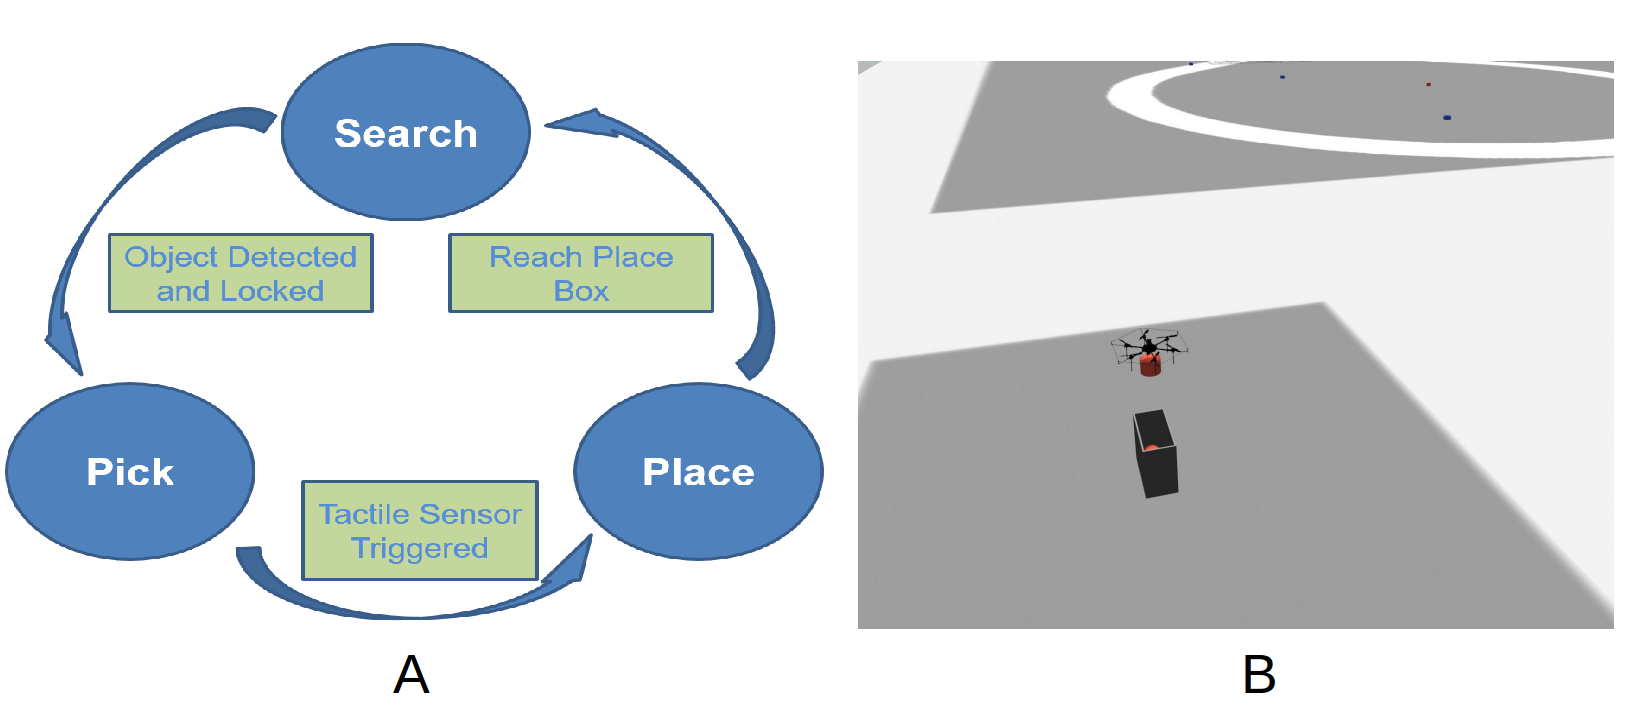
\includegraphics[keepaspectratio=true, width=1\linewidth, height=0.30\textheight]{img//task3.png}
    \end{center}
    \caption{Task 3 Demonstration}
    \label{t3}
  \end{figure}



\subsubsection{Treasure Detection}
As the treasures have distinct color features compared to the ground, we first tried the easiest detection method to find the treasure. 

The input the pointcloud we get from the Stereo sensor and the RGB image projection to the ground by the projection matrix. We first apply HSI filter to the pointcloud, get the treasure point candidates. Next we apply euclidean clustering to the filtered pointcloud. Euclidean clustering technique can organize points into clusters with respect to the distance feature. For $\forall p_i, p_j \in P_{hsi}$, clusters $O_i = \{p_i \in P_i\}$ and $O_j = \{p_j \in P_j\}$ are obtained by:
\begin{equation}\label{eq3-1}
min||p_i - p_j|| \geq d_{threhold} 
\end{equation}
When we get all the clusters, we apply a simple tracker to every cluster center and as we continue detect the same cluster, we will increase the weight of the tracker, the clusters that are not always being detect will be slowly forget and finally be removed from the treasure candidates vector. The UAV will lock the cluster candidate when the weight is large enough and switch into the "Pick" mode to approach the treasure.

\subsection{Results Achieved to Date}
We first perform full automatic simulation in gazebo\ref{t3}B. To fully simulate the real scene, we also manually add noise and outliers to the detection. In the simulation, our UAV can almost achieve $70s$ for per object, if three UAVs cooperate together, we believe we can do that better. For real robot, we performed test on with tele-operation control, both Hawk and transformable UAV can grasp the treasure we made and lift it to a given box. We are planing to perform more test on the real robot to justify the detection and motion planning algorithm in the simulation.


\end{document}
